\chap{Mehrfache Sensorschwellen}\label{ch.slow}

Wie im  \cref{a.tech} beschrieben können im fortgeschrittenen Modus Sensorereignisse auf drei verschiedene Arten abgefragt werden: ein Ereignis tritt ein, wenn das reflektierte Licht unter einem Schwellwert liegt (schwarz), ein Ereignis ritt ein, wenn das reflektierte Licht über einem SChwellwert liegt (weiss mit rotem Rand) und ein Ereignis tritt ein, wenn das reflektierte Licht zwischen zwei Schwellwerten liegt (dunkelgrau):

\begin{center}
\begin{tabular}{ccc}
\blk{slow-low}&\blk{slow-mid}&\blk{slow-high}\\
\end{tabular}
\end{center}

\textbf{Spezifikation}

Erstellen Sie ein Programm, welches den Roboter dazu bringt, sich einem Objekt zu nähern, wobei er zunächst mit hoher Geschwindigkeit fährt, dann langsamer und kurz vor dem Objekt schliesslich anhält.

\textbf{Anleitung}

\begin{itemize}
\item Verwenden Sie drei Ereignis-Aktions-Paare, je eines mit jeder der drei Arten von Sensor-Ereignissen.

\item Passen Sie die Schieberegler sorgfältig an, so dass der Schwellwert des einen Sensors dem Schwellwert des nächsten Sensors entspricht (vergleichen Sie \cref{a.tech}). 

\item Fügen Sie eine Farbe für jedes Paar ein, so dass Sie die Geschwindigkeitseinstellungen erkennen können. 

\item Verwenden Sie reflektierende Streifen wie in \cref{a.blocks} beschrieben, um die Reichweite zu erhöhen.
\end{itemize}

{\raggedleft \hfill Beispielprogramm \bu{slow.aesl}}
\bigskip

\textbf{Spezifikation}

Das ''Einer-Linie-Folgen''--Programm, das wir in  Kapitel~\ref{ch.line} gesehen haben, benutzte zwei Sensoren um zu entscheiden, ob der Roboter sich links oder rechts von der Linie entfernt. Implementieren Sie den nachfolgenden Algorithmus, der nur einen Sensor verwendet!

\textbf{Anleitung}

Der Roboter folgt der Linie dem \emph{Rand} entlang und nicht in der Mitte. Die Bodensensoren erhalten eine Reflektion aus einem relativ breiten Bereich, daher kann die Entscheidung gefällt werden mit einer Mehrfachen Sensorschwelle. Wenn der rechte Sensor verwendet wird, um der rechten Kante einer dunklen Linie zu folgen:
\begin{itemize}
	\item Wenn der Sensor zu weit links vom Rand ist, wird wenig Licht erkannt.
	\item Wenn der Sensor zu weit rechts vom Rand ist, wird viel Licht erkannt. 
	\item Wenn der Sensor über der Kante ist, wird Licht erkannt, das irgendwo zwischen den beiden Extremwerten liegt. 
\end{itemize}
Die drei Fälle werden im folgenden Diagramm dargestellt:
\begin{center}
	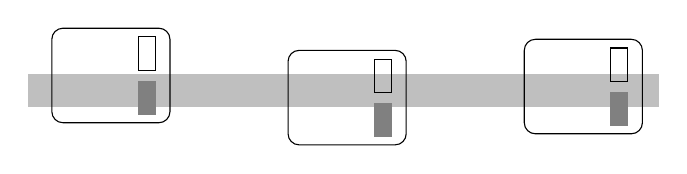
\begin{tikzpicture}
	\draw[fill,lightgray] (0,0) rectangle +(8,4mm);
	\foreach \x/\y in {6.5cm/1pt, .5cm/5pt, 3.5cm/-3pt} {
		\draw[rounded corners] (\x-2mm,\y-11pt) rectangle +(15mm,12mm);
		\draw[fill,gray] (\x+.9cm,\y-8pt) rectangle +(6pt,12pt);
		\draw (\x+.9cm,\y+8pt) rectangle +(6pt,12pt);
	}
	\end{tikzpicture}
\end{center}

\bigskip

{\raggedleft \hfill Beispielprogramm \bu{line-one.aesl}}